\documentclass[10pt,a4paper]{article}

\usepackage[a4paper,margin=2.0cm]{geometry}
\usepackage[T1]{fontenc}
\usepackage[utf8]{inputenc}
\usepackage{lmodern}
\usepackage{microtype}
\usepackage{graphicx}
\usepackage{booktabs}
\usepackage{array}
\usepackage{longtable}
\usepackage{tabularx}
\usepackage{float}
\usepackage{caption}
\usepackage{subcaption}
\usepackage{xcolor}
\usepackage{enumitem}
\usepackage{amsmath}
\usepackage[hidelinks]{hyperref}
\usepackage{placeins}

\graphicspath{{../../results/}{../../specification/}{../img/}}

\setlength{\parskip}{0.38em}
\setlength{\parindent}{0pt}
\emergencystretch=3em
\setlist[itemize]{leftmargin=1.35em,itemsep=0.2em,topsep=0.2em}
\setlist[enumerate]{leftmargin=1.45em,itemsep=0.2em,topsep=0.2em}
\captionsetup{font=small,labelfont=bf}

\newcommand{\kn}{\ensuremath{\mathrm{kn}}}
\newcommand{\ms}{\ensuremath{\mathrm{m/s}}}
\newcommand{\kw}{\ensuremath{\mathrm{kW}}}
\newcommand{\co}{CO$_2$}
\newcommand{\hs}{$H_s$}
\newcommand{\sog}{SOG}
\newcommand{\cog}{COG}
\newcommand{\alphaabs}{$|\alpha|$}

\title{\textbf{Wind-Assisted Propulsion on North Sea Routes}\\
\large Maritime Performance Analytics for Flettner Rotors}
\author{Aleksandra K\l{}os \and Olga Grigorieva \and Elen Mouradian \and Bartosz Maj \and Hubert Jaczy\'nski}
\date{DataWaves Innovation Laboratory \\
Preliminary project report, May 2026}

\begin{document}
\pagenumbering{gobble}

\begin{titlepage}
    \centering
    \vspace*{1.2cm}
    {\Huge\bfseries Wind-Assisted Propulsion on North Sea Routes\par}
    \vspace{0.35cm}
    {\Large Maritime Performance Analytics for Flettner Rotors\par}
    \vspace{0.9cm}
    {\large DataWaves Innovation Laboratory -- Preliminary project report\par}
    \vspace{0.25cm}
    {\large May 2026\par}
    \vspace{1.2cm}
    {\large
    Aleksandra K\l{}os\\
    Olga Grigorieva\\
    Elen Mouradian\\
    Bartosz Maj\\
    Hubert Jaczy\'nski\par}
\end{titlepage}

\pagenumbering{arabic}
\tableofcontents
\clearpage

\section{Executive summary}

The project studies how wind, waves, currents, and vessel heading influence
operational speed on North Sea routes, and whether Flettner rotors can improve
voyage performance or enlarge useful weather windows. The work follows the
advanced variant of the project card: AIS position reports were merged with ERA5
wind fields and Copernicus Marine sea-state/current variables, transformed into
trajectory-aware features, modelled with leakage-aware train/test splits, and
used in a rotor-assisted what-if simulation.

The final engineered dataset contains 125,160 AIS-metocean observations from
528 voyages between 2023-02-02 and 2026-02-02. The speed target is
\sog{} in knots. The modelling split is chronological by voyage: 422 voyages
and 88,346 rows are used for training; 106 later voyages and 35,758 rows are
held out for testing. This design prevents observations from the same voyage
from appearing on both sides of the split and avoids temporal leakage.

Four model levels were evaluated. A constant-speed baseline gives MAE
1.388 \kn{} and RMSE 1.893 \kn{}. A linear model using wind, wave height, and
encoded wind angle gives a small improvement, MAE 1.377 \kn{} and $R^2=0.034$.
A weather-only XGBoost model is useful for interpretation but does not improve
test accuracy under the current feature set. The best predictive model is the
lagged nowcast XGBoost model, which adds previous observed \sog{} and apparent
wind context; it reaches MAE 0.406 \kn{}, RMSE 0.758 \kn{}, $R^2=0.839$, and
91.7\% of predictions within $\pm 1$ \kn{}.

The rotor scenario is deliberately applied after prediction rather than used as
a training feature. Rotor power is estimated from the provided polar diagram and
converted to a speed increment with the repository assumption
200 \kw{} $\approx$ 1 \kn{} near the operating point. On the held-out test set,
the rotor is active in 98.1\% of observations, with mean active rotor power
41.2 \kw{}, mean active speed contribution 0.206 \kn{}, and overall mean
contribution 0.202 \kn{}. Under the weather-window definition
\sog{} $\geq 10$ \kn{} and \hs{} $\leq 3$ m, coverage increases from 76.0\% to
77.5\%. The number of separate windows decreases from 866 to 808, while points
inside windows increase by 529, suggesting that some marginal windows become
longer and merge when rotor assistance is applied.

The optional extensions add operational interpretation. The energy model
estimates 112.2 t of fuel saved and 349.4 t \co{} avoided over the three-year
dataset, or about 37.4 t fuel and 116.4 t \co{} per year. Route segmentation
shows different benefits by heading regime, with westbound legs gaining the
largest weather-window coverage increase. Route optimisation demonstrates a
Dijkstra grid-routing proof of concept for rotor gain. Gain detection shows that
only 11.9\% of observations are high-gain moments, but those moments carry a
large share of the total benefit; high gain is associated mainly with wind
speeds above 8--12 \ms{} and beam-to-quartering apparent wind angles.

\begin{table}[H]
\centering
\caption{Main quantitative outcomes from the current repository run.}
\begin{tabularx}{\textwidth}{>{\raggedright\arraybackslash}p{0.33\textwidth}X}
\toprule
\textbf{Area} & \textbf{Current result} \\
\midrule
Dataset & 125,160 observations, 528 voyages, 2023-02-02 to 2026-02-02. \\
Validation & Chronological voyage split; 422 train voyages and 106 test voyages; no temporal leakage. \\
Best speed model & XGBoost lagged nowcast: MAE 0.406 \kn{}, RMSE 0.758 \kn{}, $R^2=0.839$. \\
Rotor speed uplift & Mean active $\Delta$\sog{} 0.206 \kn{}; overall mean $\Delta$\sog{} 0.202 \kn{}. \\
Weather windows & Coverage 76.0\% without rotor and 77.5\% with rotor; +529 test observations inside windows. \\
Fuel and emissions & 112.2 t fuel saved and 349.4 t \co{} avoided over the dataset; annualised 37.4 t fuel and 116.4 t \co{}. \\
High-gain moments & 11.9\% of observations have $\Delta$\sog{} $\geq 0.5$ \kn{}; classifier F1 = 0.992. \\
\bottomrule
\end{tabularx}
\end{table}

\section{Project context and objectives}

Commercial vessels increasingly use wind-assisted propulsion to reduce fuel
burn, emissions, and exposure to volatile fuel prices. A Flettner rotor is a
rotating vertical cylinder. When wind flows around it, the Magnus effect creates
an aerodynamic lift force. Depending on the apparent wind angle and the vessel's
course, part of this force can point forward and support the main engine. In
practice the contribution is highly conditional: the same rotor can be useful,
neutral, or even unfavourable depending on wind speed, angle, sea state, vessel
speed, and operational constraints.

The project card defines the problem as an algorithmic analysis of vessel traces
and metocean conditions. The expected outputs are dependencies between
environmental conditions and voyage parameters, a scenario comparison between
baseline and rotor-assisted operation, and an assessment of weather windows for
sailing. The advanced version asks for current/tide vectors, apparent wind
calculation, rotor modelling, weather-window estimation, and uncertainty
analysis. The repository implements each of these elements.

The practical goal is not to build a final naval-architecture simulator. Instead,
the goal is to create a transparent decision-support prototype that can answer
questions such as:

\begin{itemize}
    \item How accurately can \sog{} be predicted from forecast-available
    metocean variables and recent vessel behaviour?
    \item Which environmental variables appear to influence speed under the
    current data and modelling setup?
    \item Under what wind-speed and wind-angle combinations do rotors provide
    meaningful operational gain?
    \item Do rotors increase the fraction of time in which a voyage satisfies a
    useful weather-window criterion?
    \item Can energy, \co{}, route segmentation, and routing analyses be built
    consistently on top of the same feature set?
\end{itemize}


\section{Data sources and preprocessing}

\subsection{Raw inputs}

The core input is a set of AIS-derived position reports for the analysed vessel.
Each point contains time, latitude, longitude, speed over ground, course over
ground, and trajectory-derived distance fields. These observations are enriched
with gridded metocean data from numerical models:

\begin{itemize}
    \item ERA5 wind variables: 10 m wind components and gust information.
    \item Copernicus Marine sea state: significant wave height, mean wave
    direction, and mean wave period.
    \item Copernicus Marine currents: eastward and northward current components.
\end{itemize}

The merged \texttt{MasterSet.csv} file contains the base AIS-metocean table.
The engineered feature file contains the modelling
features used by the baseline and extension notebooks. The feature-engineering
notebook reports 125,160 rows and 57 columns after processing.

\subsection{Spatio-temporal alignment}

AIS points are irregular in time and space, while metocean products are gridded.
The preprocessing pipeline aligns these sources by interpolating environmental
variables to each AIS position and timestamp. This is the key step that turns a
vessel trajectory into a supervised learning table. For each AIS observation the
pipeline attaches the environmental state that the vessel experienced at that
location and time.

The repository separates this work across proof-of-concept interpolation,
ERA5-checking, exploratory-analysis, and feature-engineering notebooks. The
resulting dataset spans 2023-02-02 to 2026-02-02 and covers 528 voyages.

\begin{figure}[H]
    \centering
    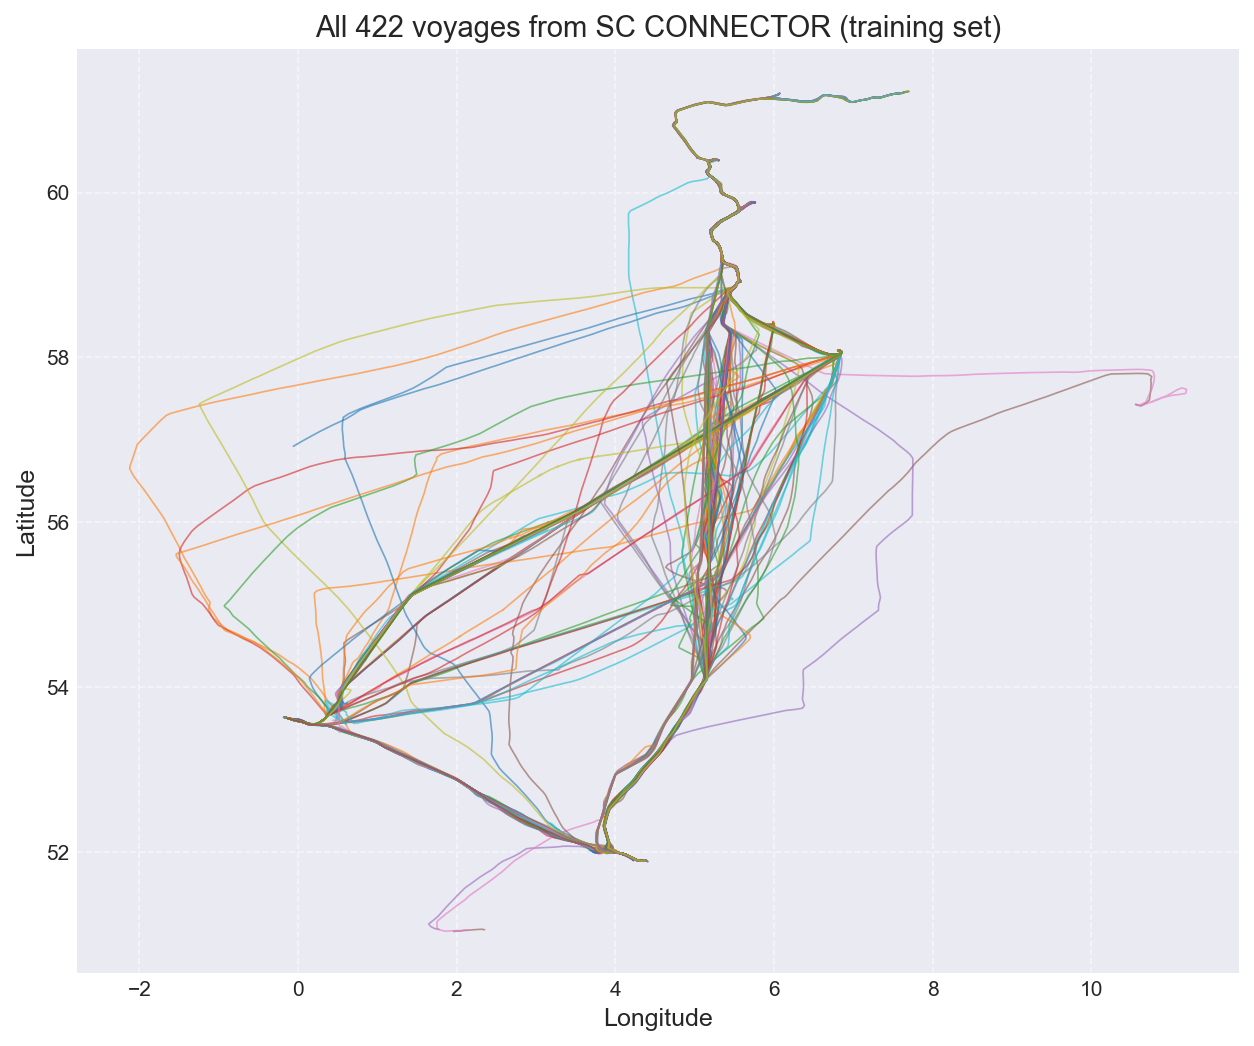
\includegraphics[width=0.74\textwidth]{all_trajectories.png}
    \caption{Training trajectories used by the project pipeline.}
\end{figure}

\subsection{Feature engineering}

The engineered variables follow a leakage-aware design. Features are divided
into explanatory metocean/route variables, lagged nowcast variables, and
post-prediction rotor-scenario variables. The main feature groups are:

\begin{itemize}
    \item \textbf{Wind and wave features}: true wind speed, significant wave
    height \hs{}, wave period, wind speed squared, and wave-wind alignment.
    \item \textbf{Relative-angle features}: wind direction and angle relative to
    vessel course, encoded with sine/cosine terms to avoid discontinuity at
    0/360 degrees.
    \item \textbf{Apparent wind features}: apparent wind speed and apparent
    relative angle, reserved for the nowcast model.
    \item \textbf{Current features}: current magnitude, current direction, and
    along-course/cross-course current components.
    \item \textbf{Lagged target features}: previous \sog{}, two-step previous
    \sog{}, and a shifted rolling mean over up to three previous observations.
    \item \textbf{Interaction terms}: wind-angle, apparent-wind-angle,
    wind-wave, nonlinear wind/wave terms, and current-course interactions.
\end{itemize}

The most important leakage control is that the shifted rolling mean never uses
the current target row. The lag features are grouped by voyage, so the first
observations in a voyage do not inherit speed information from a previous
voyage. This makes the nowcast model realistic for short-horizon prediction
while keeping the weather-only model interpretable.

\begin{table}[H]
\centering
\caption{Representative variables in the engineered feature table.}
\begin{tabularx}{\textwidth}{>{\raggedright\arraybackslash}p{0.24\textwidth}X}
\toprule
\textbf{Group} & \textbf{Examples and role} \\
\midrule
Trajectory & \texttt{Time}, \texttt{Lat}, \texttt{Lon}, \texttt{Voyage\_ID}, \texttt{Course\_deg}, \texttt{Dist\_since\_last\_nm}. \\
Target & \texttt{Speed\_kn}; the predicted speed over ground. \\
Wind/wave & \texttt{True\_Wind\_Speed\_ms}, \texttt{H\_s}, \texttt{mwp}, \texttt{fg10}, wave-wind alignment. \\
Angles & \texttt{alpha\_sin}, \texttt{alpha\_cos}, apparent wind angle encodings. \\
Currents & \texttt{Current\_Speed\_ms}, along-course and cross-course current terms. \\
Nowcast history & \texttt{Speed\_kn\_lag1}, \texttt{Speed\_kn\_lag2}, \texttt{Speed\_kn\_mean3}. \\
Rotor scenario & Rotor power, active flag, and $\Delta$\sog{} are used after model prediction, not as training features. \\
\bottomrule
\end{tabularx}
\end{table}

\section{Methodology}

\subsection{Speed prediction problem}

The primary supervised learning target is vessel speed over ground:

\[
\widehat{\sog}_t = f(X_t),
\]

where $X_t$ contains environmental variables, route context, and, for the
nowcast model only, previous observed speed. The models are evaluated on later
voyages that were not used for training. This is essential because random row
splits would allow neighbouring points from the same voyage to appear in both
train and test sets, giving overly optimistic performance.

The project uses three conceptual model families:

\begin{enumerate}
    \item \textbf{B1 constant mean}: predicts the mean training speed for every
    test observation.
    \item \textbf{B2 linear weather model}: predicts speed from true wind speed,
    \hs{}, and sine/cosine encoding of the relative wind angle.
    \item \textbf{XGBoost models}: gradient-boosted trees trained in two modes:
    weather-only explanatory modelling and lagged nowcast prediction.
\end{enumerate}

The XGBoost implementation uses 300 estimators, maximum depth 6, learning rate
0.05, 80\% row subsampling, 80\% column subsampling, and a fixed random seed.
Features are standardised before model fitting in the current notebook
implementation.

\subsection{Weather-only versus nowcast modelling}

The report distinguishes two purposes that are easy to confuse:

\begin{itemize}
    \item The \textbf{weather-only model} is an explanatory model. It excludes
    target-history features, so its behaviour is more directly related to
    wind, waves, currents, and route context.
    \item The \textbf{lagged nowcast model} is a predictive operational model.
    It uses previous speed observations and apparent wind context, making it
    much more accurate for short-horizon prediction.
\end{itemize}

This separation matters for interpretation. A high-performing nowcast model can
mostly learn persistence: ships tend to continue moving near their recent speed.
That is useful operationally, but it does not by itself prove that weather
features are strongly explanatory. The repository therefore reports both model
types and treats weather interpretation with caution.

\subsection{Rotor scenario model}

The rotor scenario is applied after baseline speed prediction. For each AIS
observation, the rotor utility estimates a propulsion power
$P_\mathrm{rotor}$ from wind speed and relative wind angle using the supplied
polar-response table. The rotor is active if:

\[
P_\mathrm{rotor} > 0,\quad H_s \leq 6 \mathrm{\ m},\quad
U_\mathrm{wind} \leq 42 \mathrm{\ m/s}.
\]

The speed contribution is then approximated as:

\[
\Delta \sog = \frac{P_\mathrm{rotor}}{200 \kw / \kn}
\]

when the rotor is active, otherwise $\Delta \sog = 0$. This is a transparent
surrogate assumption rather than a full hydrodynamic propulsion model. Its value
is that it makes the scenario auditable: the rotor benefit can be traced back to
the wind-speed/angle polar, wave-height gate, and a single power-to-speed
conversion.

\subsection{Weather-window definition}

The main weather-window criterion follows the project card:

\[
\sog \geq 10 \kn \quad \mathrm{and} \quad H_s \leq 3 \mathrm{\ m}.
\]

For every test-set observation the pipeline compares a baseline prediction
against a rotor-assisted prediction. Contiguous observations satisfying the
criterion form weather windows. The report tracks both the number of windows and
the number/share of observations inside windows. Counting both is important:
the rotor can reduce the number of separate windows if neighbouring windows
merge into longer continuous periods.

\subsection{Uncertainty evaluation}

The baseline notebook also trains quantile-regression prediction intervals for
the nowcast speed model. The reported 95\% interval has mean lower bound
9.670 \kn{}, mean upper bound 12.831 \kn{}, mean width 3.161 \kn{}, and empirical
coverage 96.5\% on the test set. This suggests that the interval model is
slightly conservative but well calibrated for the current test distribution.


\section{Model results and evaluation}

\subsection{Dataset split}

The train/test split is chronological by voyage. The first 80\% of voyages by
start time are used for training; the final 20\% are used for testing. The
baseline notebook reports:

\begin{itemize}
    \item Training set: 88,346 rows from 422 voyages.
    \item Test set: 35,758 rows from 106 voyages.
    \item Training period: 2023-02-02 to 2025-05-23.
    \item Test period: 2025-05-23 to 2026-02-02.
    \item Temporal leakage check: true.
\end{itemize}

This split is stricter than a random split and is therefore a stronger estimate
of generalisation to future voyages.

\subsection{Regression metrics}

The model comparison is summarised in Table~\ref{tab:model-metrics}. The
constant mean and linear weather model are close to one another. The weather-only
XGBoost model performs poorly relative to the linear baseline on the held-out
test period, which suggests either distribution shift, missing operational
variables, or that a large part of speed variation is driven by control decisions
and vessel state not visible in the current feature table. The lagged nowcast
model is much stronger because recent observed speed is a powerful predictor.

\begin{table}[H]
\centering
\caption{Held-out test performance for the core model hierarchy.}
\label{tab:model-metrics}
\begin{tabular}{lrrrr}
\toprule
\textbf{Model} & \textbf{MAE [\kn]} & \textbf{RMSE [\kn]} & \textbf{$R^2$} & \textbf{Within $\pm 1$ \kn} \\
\midrule
B1: Constant mean & 1.388 & 1.893 & -0.002 & 49.3\% \\
B2: Linear wind/wave/angle & 1.377 & 1.860 & 0.034 & 49.5\% \\
M1: XGBoost weather-only & 1.468 & 1.883 & 0.010 & 41.7\% \\
M2: XGBoost lagged nowcast & 0.406 & 0.758 & 0.839 & 91.7\% \\
\bottomrule
\end{tabular}
\end{table}

\begin{figure}[H]
    \centering
    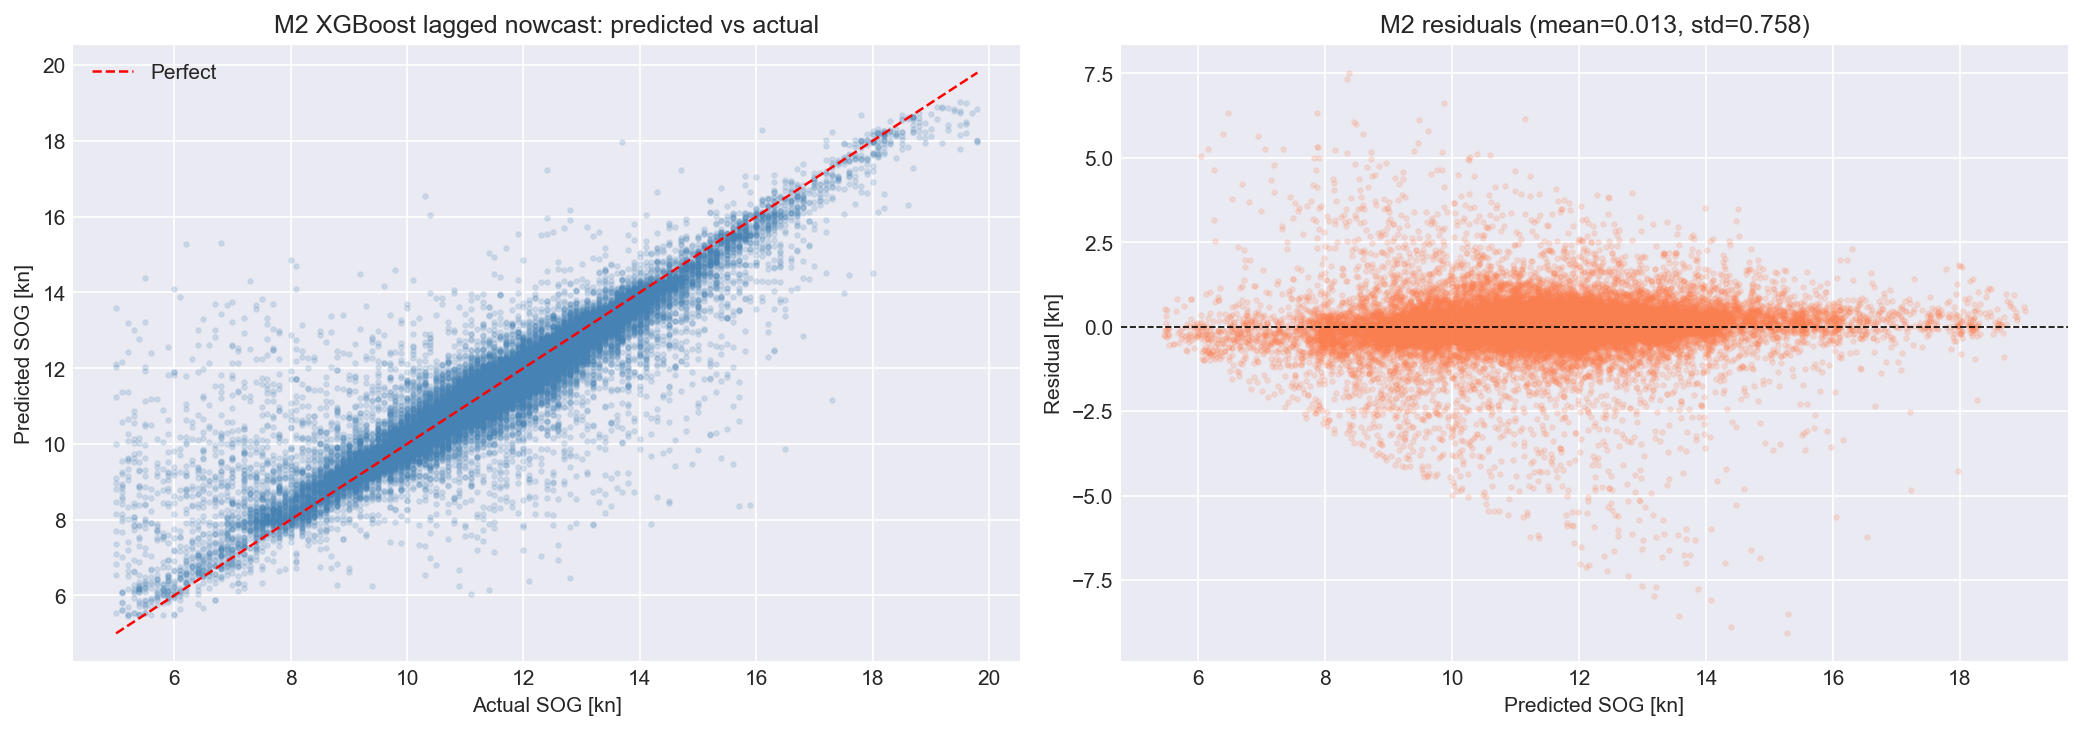
\includegraphics[width=0.78\textwidth]{predicted_vs_actual.png}
    \caption{Predicted versus actual \sog{} for the lagged nowcast model.}
\end{figure}

\subsection{Feature importance}

The weather-only model ranks course and current interaction terms highly, while
the lagged nowcast model is dominated by recent observed speed. This is
consistent with vessel operations: the current speed carries information about
engine setting, traffic, manoeuvring, loading, and other operational factors
that are not explicitly modelled.

\begin{figure}[H]
    \centering
    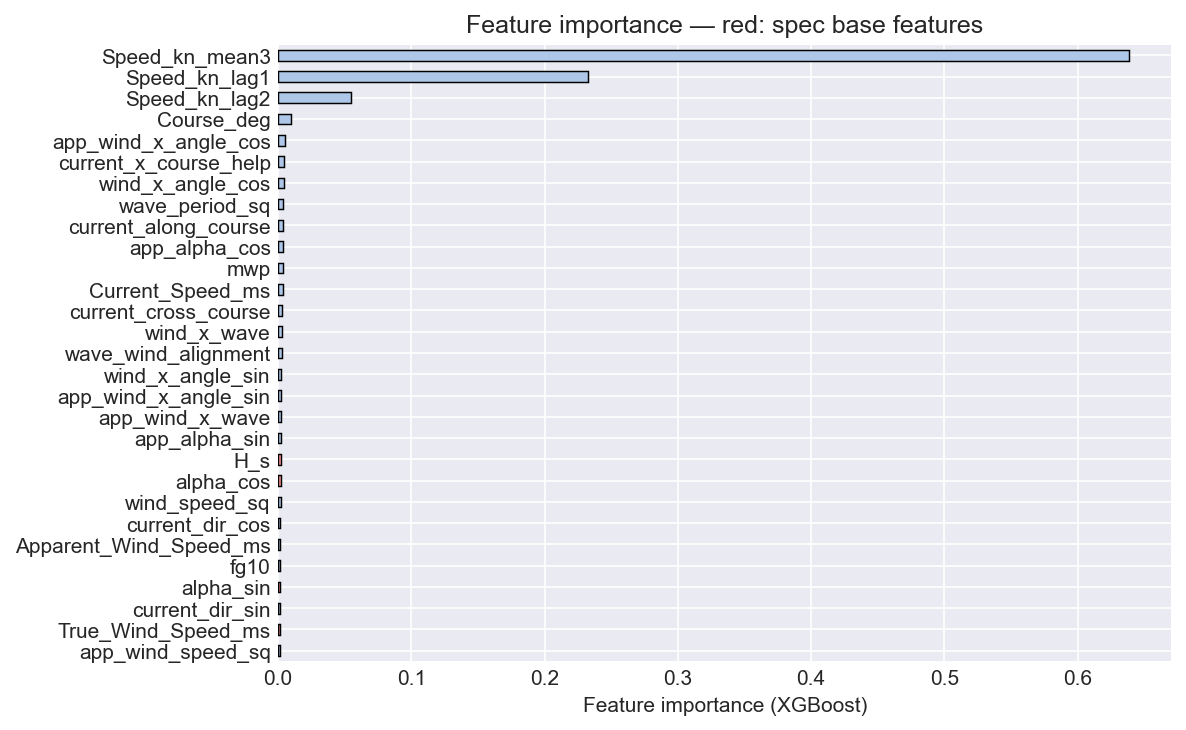
\includegraphics[width=0.82\textwidth]{feature_importance.png}
    \caption{Feature importances for weather-only and lagged nowcast XGBoost
    models.}
\end{figure}

The main interpretation is therefore twofold. First, the project can now predict
short-term \sog{} accurately when recent speed is available. Second, pure
weather-to-speed inference is harder than expected and should be treated as an
explanatory sensitivity tool rather than a final operational predictor.

\section{Rotor and weather-window results}

\subsection{Rotor what-if scenario}

On the test set, the rotor surrogate is active for 35,077 of 35,758 rows, or
98.1\% of observations. The mean rotor power when active is 41.2 \kw{}. The mean
active speed increment is 0.206 \kn{}, and the overall mean increment is
0.202 \kn{}. Per-voyage results are heterogeneous: the highest-gain voyages in
the test set show mean speed contributions from about 0.47 \kn{} to 1.19 \kn{},
while the overall mean remains modest because many observations have weaker
wind, less favourable angle, or low rotor power.

\begin{figure}[H]
    \centering
    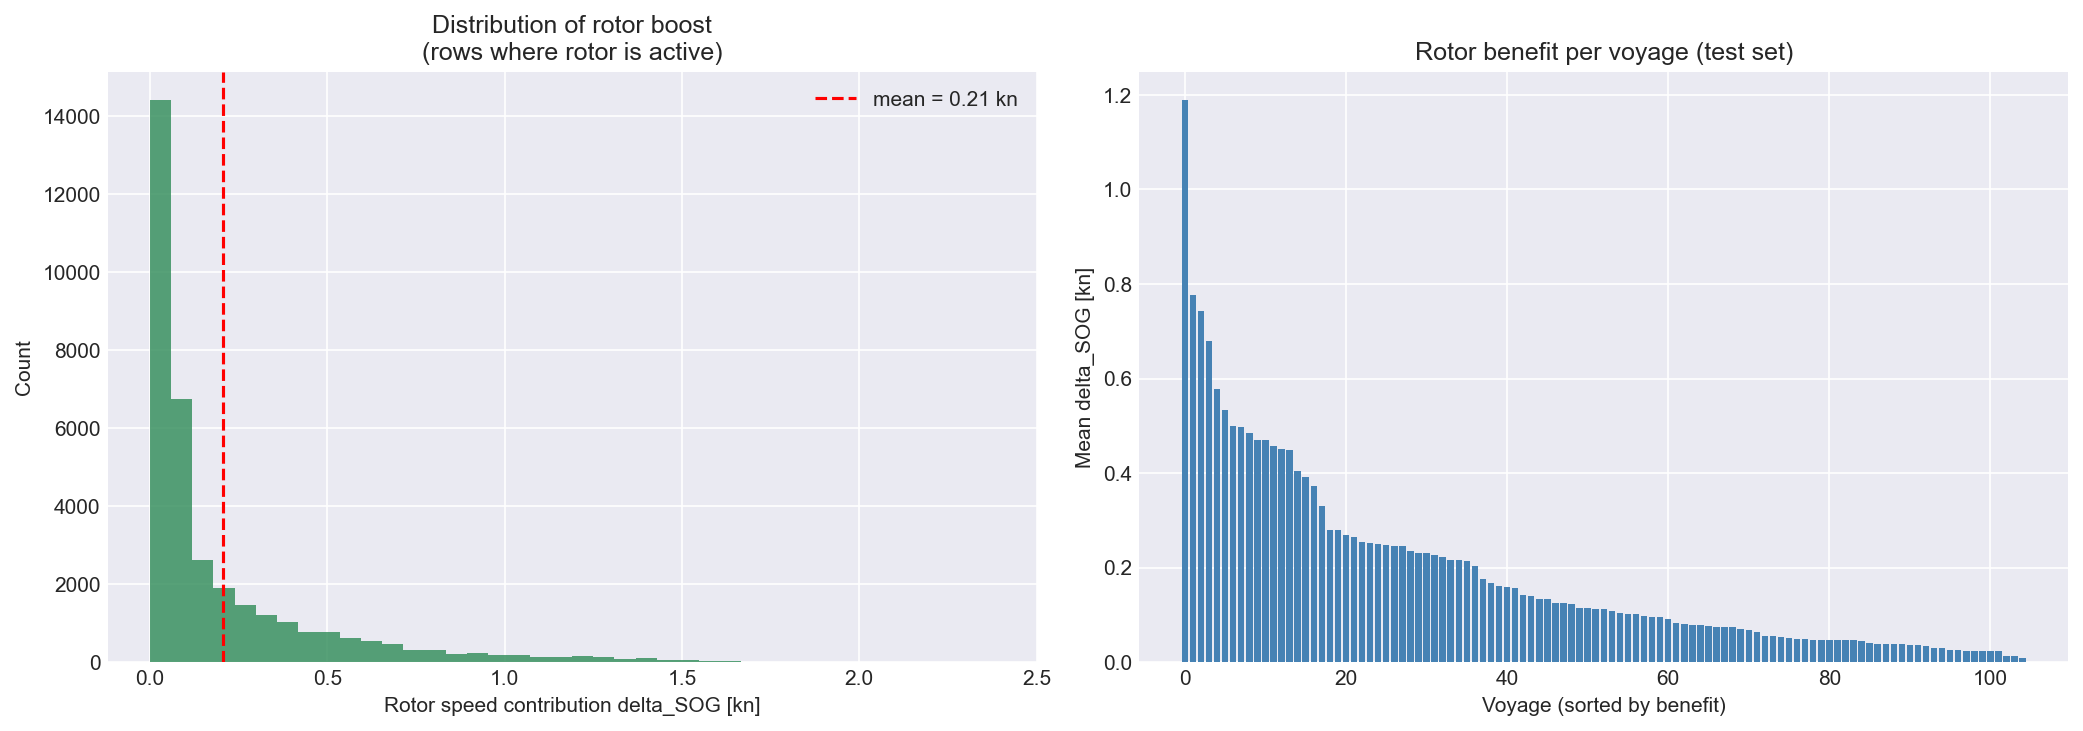
\includegraphics[width=0.78\textwidth]{rotor_scenario.png}
    \caption{Rotor scenario distribution and per-voyage mean speed contribution.}
\end{figure}

The result is operationally meaningful but not spectacular in average speed
terms. An average 0.2 \kn{} speed uplift can still matter over long voyages,
especially if it moves marginal periods over a speed threshold or allows lower
engine load for the same schedule. The larger gains occur in a smaller subset of
conditions, which motivates the gain-detection extension.

\subsection{Weather-window impact}

The weather-window analysis evaluates whether rotor assistance helps maintain
the criterion \sog{} $\geq 10$ \kn{} and \hs{} $\leq 3$ m. The result is:

\begin{table}[H]
\centering
\caption{Weather-window comparison on the held-out test set.}
\begin{tabular}{lrrr}
\toprule
\textbf{Scenario} & \textbf{Windows} & \textbf{Points in window} & \textbf{Coverage} \\
\midrule
Without rotor & 866 & 27,167 & 76.0\% \\
With rotor & 808 & 27,696 & 77.5\% \\
Delta & -58 & +529 & +1.5 percentage points \\
\bottomrule
\end{tabular}
\end{table}

The decrease in the number of windows should not be read as a negative result.
When rotor assistance lifts speed above the threshold between two favourable
periods, separate windows can merge. The more relevant operational result is
that the number of points inside the window increases and total coverage rises.

\subsection{High-gain geography and environmental structure}

The gain-surface and interaction plots show that rotor benefits cluster in
particular wind-speed and angle regimes. This is expected from the polar diagram:
headwind and tailwind directions are poor, while beam and broad-reaching angles
are stronger. Wave height mostly acts as a boundary or risk condition; in the
implemented scenario the rotor is forced off above \hs{} = 6 m, and only 19
observations exceed that threshold in the full engineered dataset.

\begin{figure}[H]
    \centering
    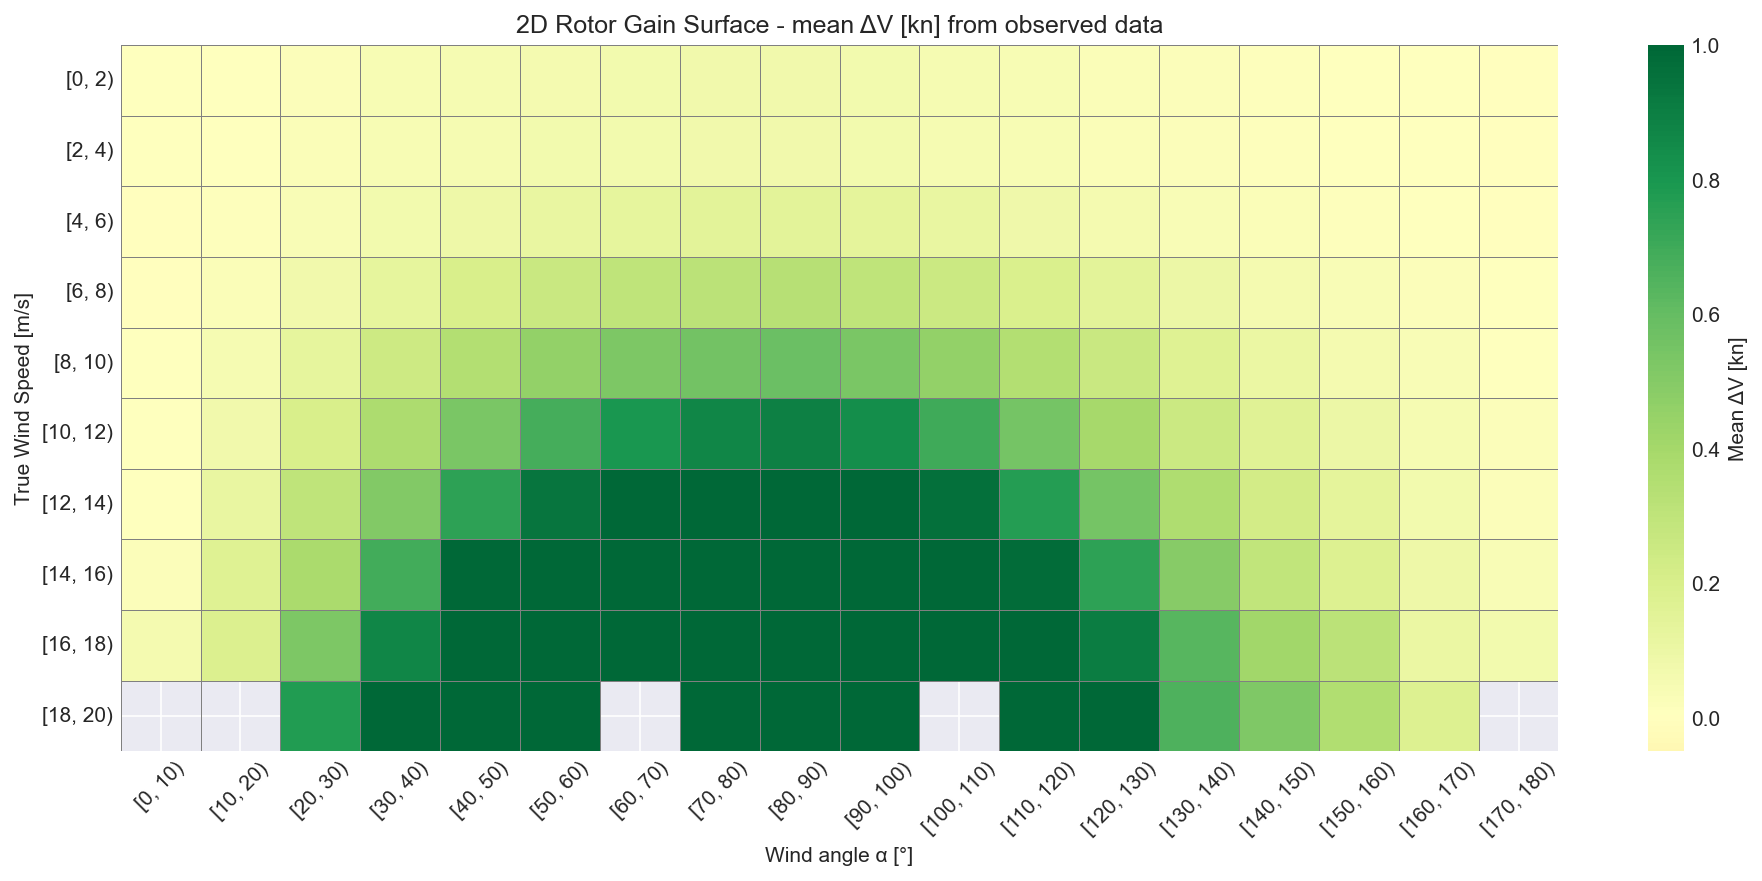
\includegraphics[width=0.68\textwidth]{rotor_gain_surface.png}
    \caption{Environmental structure of the rotor-gain scenario.}
\end{figure}

\section{Energy, emissions, and CII extension}

The first extension converts rotor power into an energy and emissions impact.
The ship model assumes 3,500 \kw{} at design speed 11.5 \kn{}, a cubic
resistance relationship, specific fuel oil consumption of 195 g/kWh, and an HFO
\co{} factor of 3.114 t \co{}/t fuel. Under these assumptions the fuel rate at
design speed without the rotor is 16.38 t/day.

The three-year dataset summary is:

\begin{itemize}
    \item Total observations: 125,160.
    \item Rotor active share: 97.6\%.
    \item Mean brake power: 3,887 \kw{}.
    \item Mean rotor power when active: 40.4 \kw{}.
    \item Total fuel baseline: 11,066.7 t.
    \item Total fuel with rotor: 10,954.4 t.
    \item Fuel saved: 112.2 t, or 1.01\%.
    \item \co{} saved: 349.4 t, or 1.01\%.
\end{itemize}

\begin{figure}[H]
    \centering
    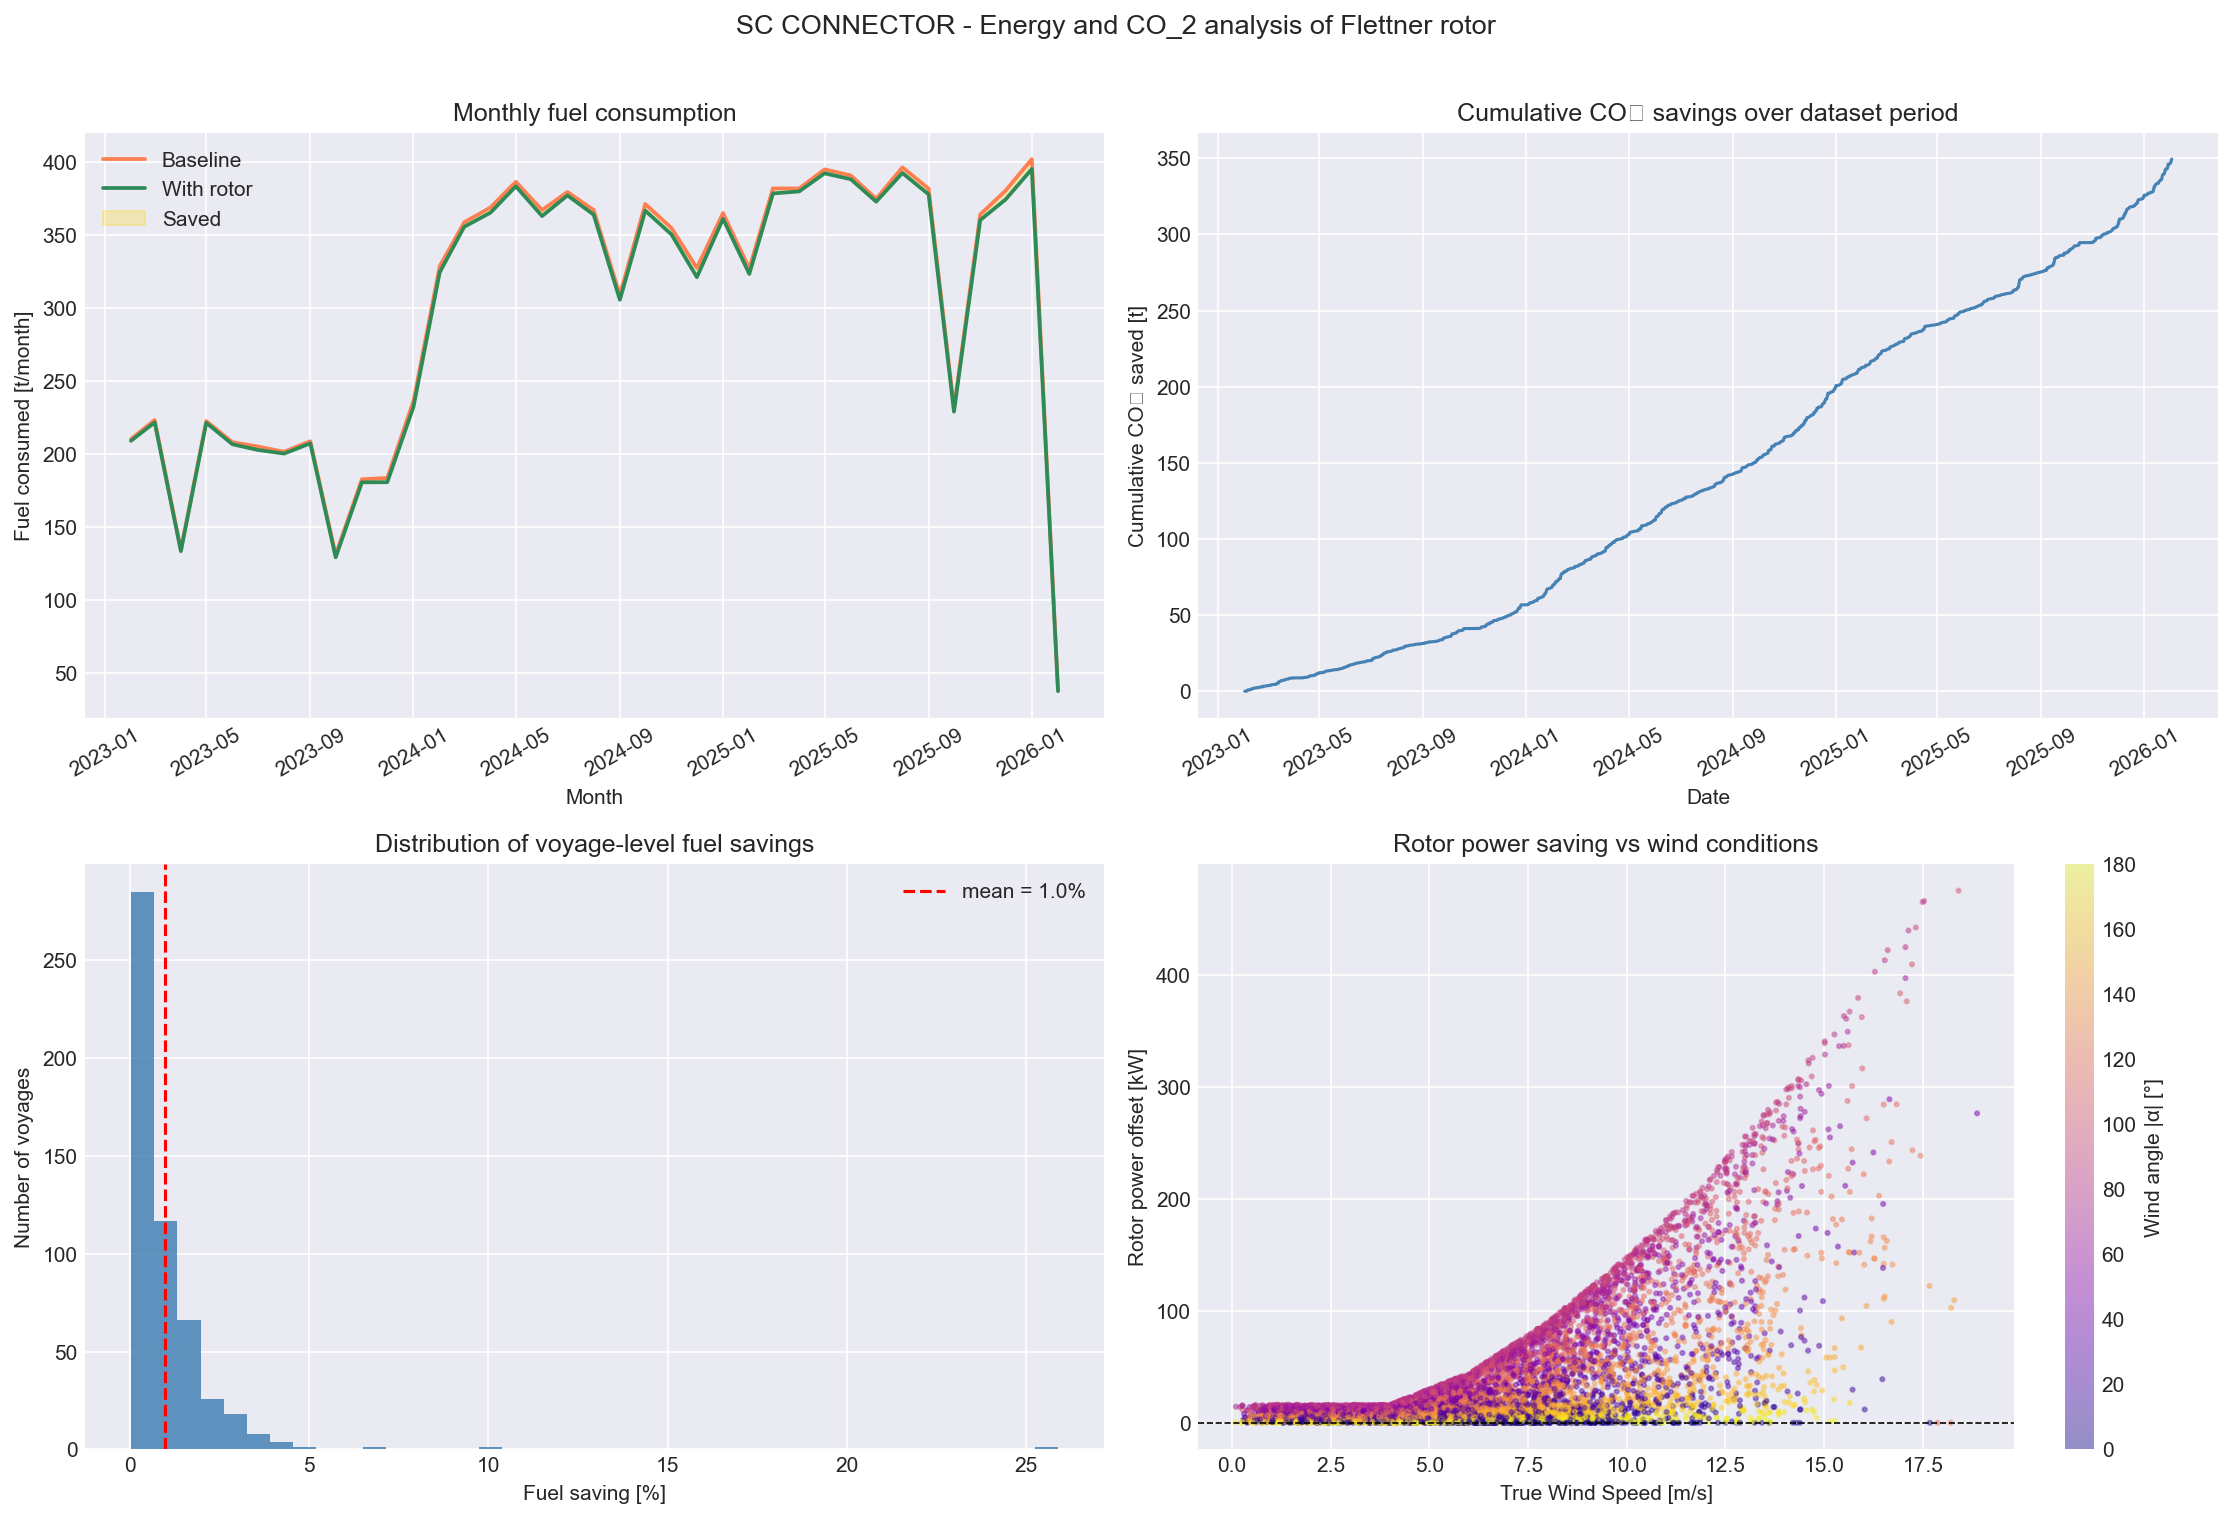
\includegraphics[width=0.78\textwidth]{energy_fuel_co2.png}
    \caption{Fuel and \co{} impact estimated from the rotor energy model.}
\end{figure}

Annualised over the dataset duration of 1,096 days, the extension estimates
37.4 t fuel saved per year and 116.4 t \co{} avoided per year. The attained CII
estimate improves from 53.75 to 53.20 g \co{}/(t nm), a 1.01\% improvement.

The conclusion is that the average annual energy impact is modest for one rotor,
but it is measurable and directionally useful. The result should be interpreted
as an order-of-magnitude scenario rather than a guaranteed vessel-performance
claim, because the model does not yet include detailed propeller curves, engine
load-specific SFOC, hull fouling, loading condition, RPM control policy, or
captain/charterer speed decisions.

\section{Route segmentation extension}

Route segmentation divides the data into heading regimes: northbound,
eastbound, southbound, and westbound. This makes the analysis more interpretable
because rotor performance is strongly tied to the relationship between course
and wind. A single global model can hide differences between legs moving through
different prevailing-wind relationships.

\begin{table}[H]
\centering
\caption{Regime-level characterisation from the full dataset.}
\begin{tabular}{lrrrr}
\toprule
\textbf{Regime} & \textbf{Mean \sog{} [\kn]} & \textbf{Mean wind [\ms]} & \textbf{Mean \hs{} [m]} & \textbf{Mean $\Delta$\sog{} [\kn]} \\
\midrule
Northbound & 12.05 & 7.0 & 1.32 & 0.209 \\
Eastbound & 12.34 & 6.2 & 1.06 & 0.185 \\
Southbound & 10.95 & 6.8 & 1.28 & 0.196 \\
Westbound & 10.58 & 6.5 & 1.21 & 0.209 \\
\bottomrule
\end{tabular}
\end{table}

The per-regime weather-only XGBoost models show mixed predictive quality.
Northbound has the lowest MAE at 1.219 \kn{}, while westbound is hardest to
predict at MAE 1.788 \kn{}. Eastbound is the only regime with clearly positive
$R^2$ in the per-regime model summary, $R^2=0.137$, while the other regimes have
negative $R^2$. This again supports the conclusion that weather-only
generalisation is difficult.

The most useful output from this extension is the weather-window effect by
heading. Westbound legs improve from 85.1\% to 90.1\% coverage, the largest
regime-level gain. Southbound improves from 82.3\% to 84.5\%. Northbound and
eastbound already have high baseline coverage and therefore show smaller
coverage changes.

\section{Route optimisation extension}

The route-optimisation extension explores whether route choice can increase the
expected rotor benefit. The implemented proof of concept builds a coarse
0.5-degree spatial grid from historical metocean/rotor-gain fields and applies
Dijkstra search to identify a path with improved integrated rotor gain. The
reference voyage is Voyage 456, from approximately 51.89 degrees N, 4.40
degrees E to 61.23 degrees N, 7.68 degrees E. The great-circle distance is about
570.7 nm.

The spatial field contains 72 grid cells with data. Mean rotor power across the
grid is 78.5 \kw{}, and the best historical cells reach mean rotor powers above
180--290 \kw{} under favourable conditions. The route-search result reports an
optimal path of 19 nodes, distance 568.0 nm versus 571.0 nm for the direct grid
path, mean rotor power 7.5 \kw{} versus 1.9 \kw{} direct, and mean
$\Delta$\sog{} 0.037 \kn{} versus 0.010 \kn{} direct. Relative improvement is
large at +288.5\%, but the absolute gain in this specific route experiment is
small.

\begin{figure}[H]
    \centering
    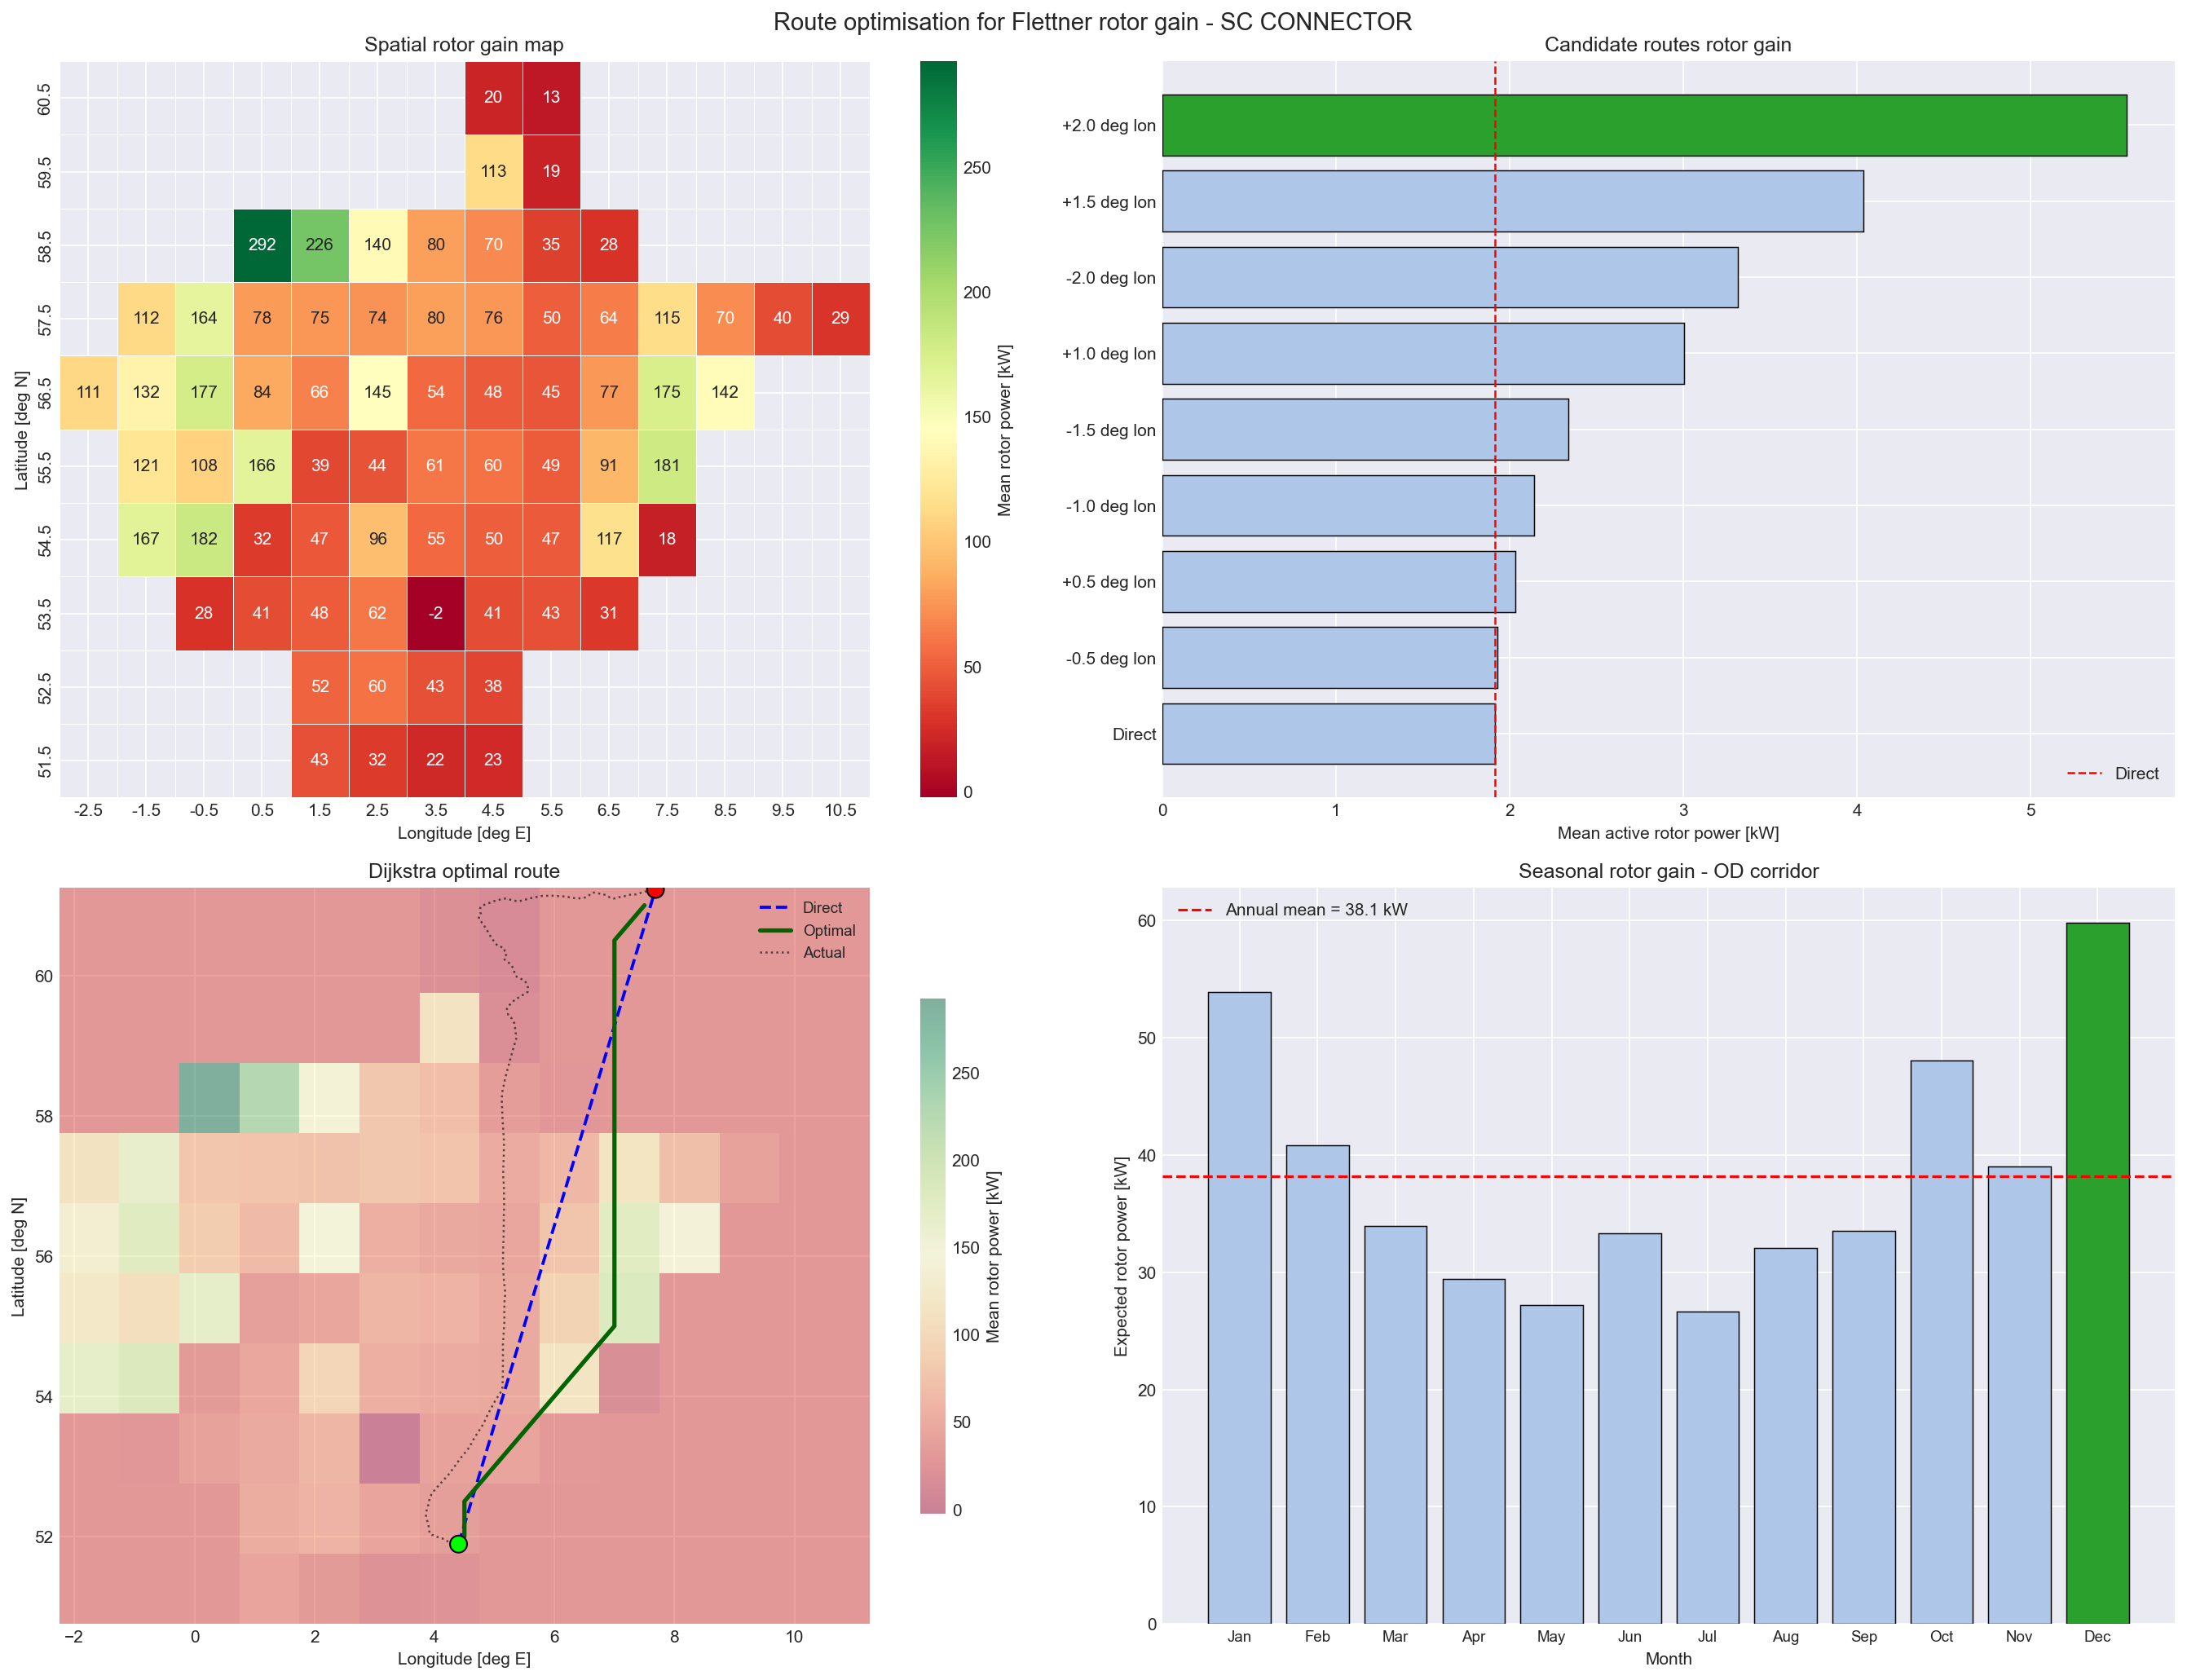
\includegraphics[width=0.78\textwidth]{route_optimization.png}
    \caption{Dijkstra-based routing proof of concept for rotor-gain optimisation.}
\end{figure}

The extension also studies seasonal sensitivity. December has the best expected
monthly rotor power, 59.8 \kw{}, while July is worst at 26.6 \kw{}. The seasonal
pattern is intuitive for the North Sea: winter has stronger winds, but it may
also have more severe waves and operational risk. A final routing product should
therefore optimise a multi-objective score, not rotor gain alone. A practical
score would combine expected arrival time, fuel, \co{}, wave limits, route
deviation, safety margin, and schedule reliability.

\section{Rotor gain detection extension}

The gain-detection extension turns the rotor scenario into a classification and
decision problem. A high-gain observation is defined as
$\Delta$\sog{} $\geq 0.5$ \kn{}. Under the current surrogate model, high-gain
moments account for 14,856 observations, or 11.9\% of the full dataset.

Rotor gain increases strongly with wind speed. The notebook reports mean
$\Delta$\sog{} of 0.037 \kn{} for wind below 4 \ms{}, 0.273 \kn{} for 8--10
\ms{}, 0.431 \kn{} for 10--12 \ms{}, 0.610 \kn{} for 12--14 \ms{}, and
0.897 \kn{} above 14 \ms{}. The optimal high-gain subset has median wind speed
11.5 \ms{}, and 90\% of those observations are above 9.2 \ms{}.

Angle is equally important. High-gain observations have median absolute relative
wind angle around 82 degrees, with 80\% of the main high-gain subset between 50
and 113 degrees. This matches the rotor polar: beam and quartering winds are
useful, while headwind and tailwind sectors are poor.

\begin{figure}[H]
    \centering
    \begin{subfigure}{0.48\textwidth}
        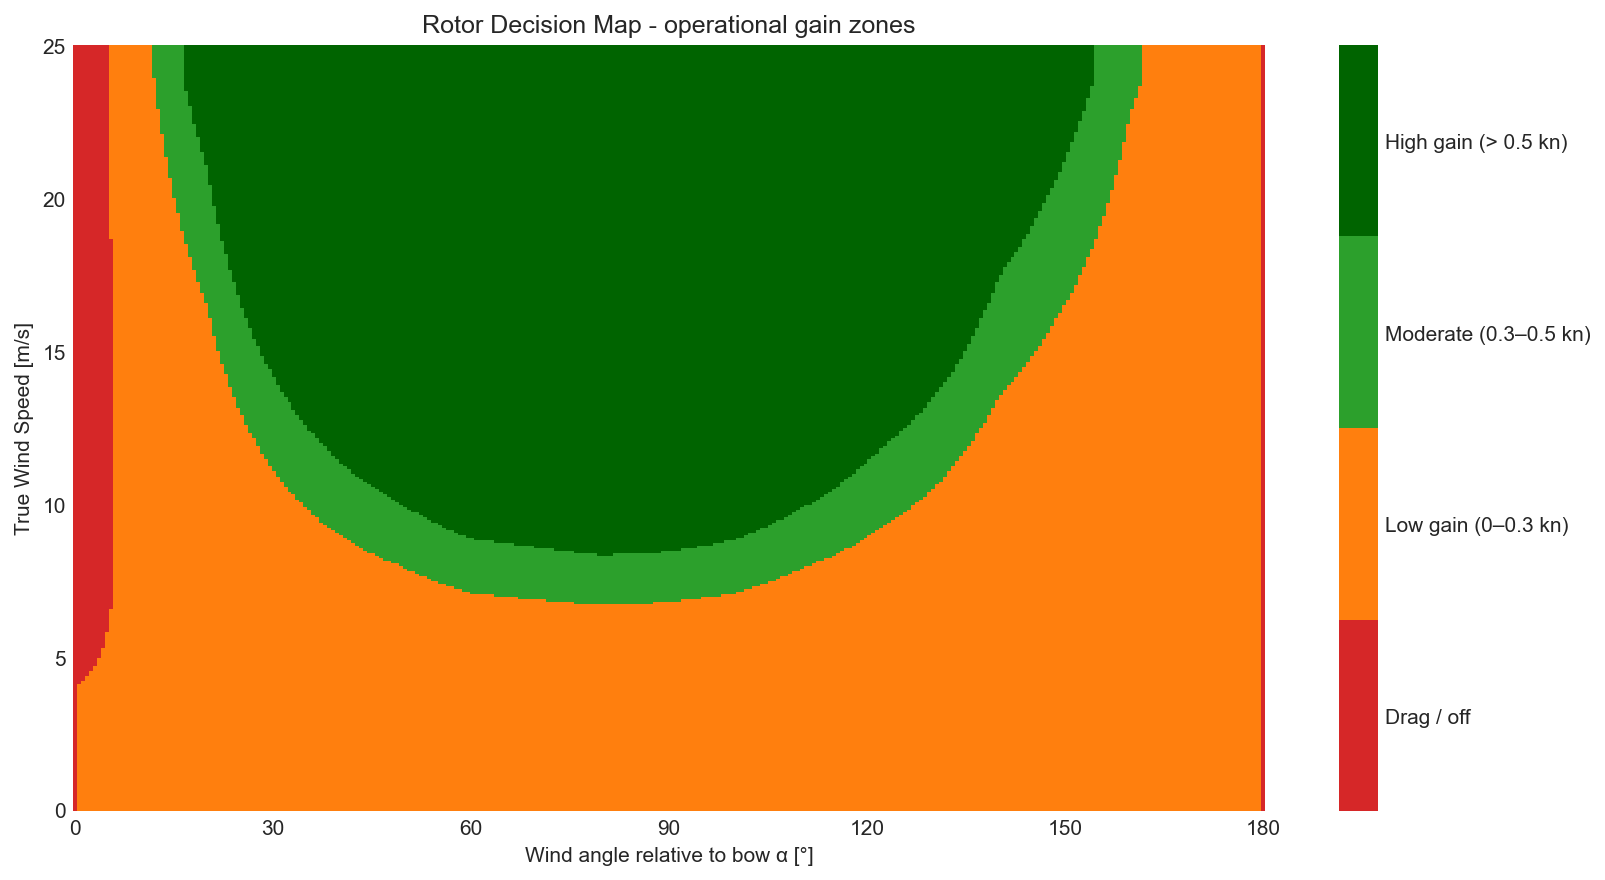
\includegraphics[width=\textwidth]{rotor_decision_map.png}
        \caption{Rule-based high-gain zones.}
    \end{subfigure}
    \hfill
    \begin{subfigure}{0.48\textwidth}
        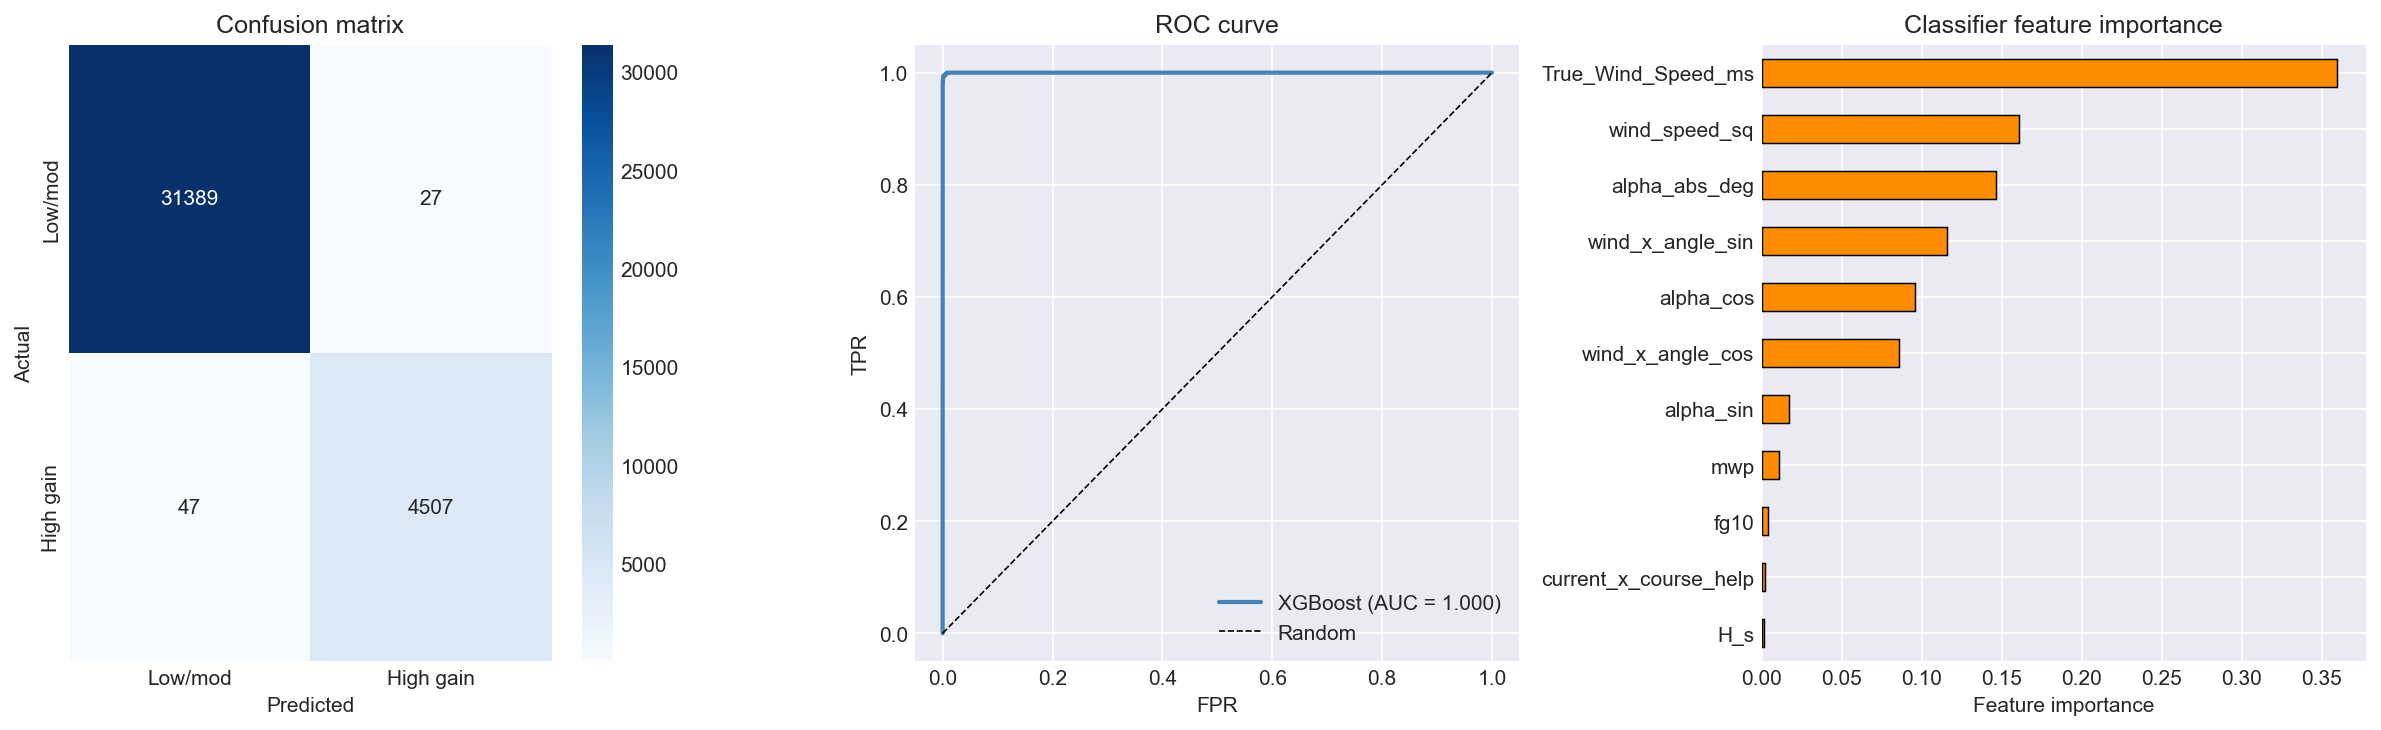
\includegraphics[width=\textwidth]{rotor_classifier.png}
        \caption{Classifier performance.}
    \end{subfigure}
    \caption{Operational detection of high-gain rotor conditions.}
\end{figure}

An XGBoost classifier identifies high-gain moments with 99.8\% accuracy,
99.4\% precision, 99.0\% recall, F1 = 0.992, and ROC-AUC = 1.000 on the
notebook split. These very high metrics are plausible because the target is
derived directly from the same rotor-power surrogate and its input variables;
the classifier is therefore best interpreted as a compact decision-rule learner,
not as independent proof of physical rotor performance.

The rule-based decision system is more transparent: if wind is at least 8 \ms{}
and angle is between 50 and 130 degrees, or wind is at least 12 \ms{} and angle
is between 40 and 140 degrees, mark high gain. This rule reaches 95.8\% recall,
69.7\% precision, and 94.2\% accuracy. For operations, the rule is attractive
because it is easy to explain and can be applied to forecasts.



\section{Conclusions}

The project has progressed beyond a simple baseline and now forms a coherent
maritime analytics prototype. AIS trajectories are enriched with wind, waves,
and currents; leakage-aware models are trained and evaluated by voyage; rotor
assistance is simulated as a transparent what-if layer; and the results are
translated into weather windows, fuel, emissions, route regimes, routing, and
high-gain operational rules.

The central technical finding is that recent vessel speed is the strongest
predictor of near-term speed. The lagged nowcast model reaches MAE 0.406 \kn{}
and $R^2=0.839$, while weather-only models remain much weaker. This distinction
should be presented honestly: the project can predict speed well in a nowcast
setting, but causal weather-only interpretation is still limited by missing
operational variables.

The central rotor finding is that the average benefit of one rotor is moderate
but operationally relevant. Mean speed uplift is about 0.2 \kn{} across the test
set, weather-window coverage increases by 1.5 percentage points, and the energy
extension estimates about 37 t/year fuel saving and 116 t/year \co{} reduction.
The most useful message is conditionality: the rotor is most valuable in a
minority of high-gain moments, especially when wind is above roughly 8--12
\ms{} and the apparent wind angle is near beam/quartering sectors.


\section{Transparency statement}
\label{sec:transparency}

This report was partly done with the assistance of generative AI tools. Mostly the paraphrasing and summarisation. 
The AI was used to help condense and clarify the technical content, but all key findings, interpretations, 
and conclusions were generated by the authors. 
The AI did not have access to the raw data or code and did not make any modelling decisions. 
The report was reviewed and edited by the authors to ensure accuracy and relevance.

\end{document}
